\documentclass[a4paper,11pt,twoside,final,titlepage,onecolumn,openright]{report}
\usepackage{fontspec} 
\usepackage[xetex]{geometry} 
\usepackage{xunicode}
\usepackage{xltxtra}
\defaultfontfeatures{Mapping=tex-text}
\setmainfont [Ligatures={Common}]{Linux Libertine O}
\usepackage{microtype} 
\usepackage[spanish]{babel}
\usepackage{csquotes}
\usepackage{graphicx}
\usepackage{amsmath}
\usepackage{textcomp}
\usepackage{fontawesome}
\usepackage{tabularx, booktabs}
\usepackage[lofdepth,lotdepth]{subfig}
\usepackage{url}
\usepackage[sorting=none, url=false, doi=true, eprint=false, isbn=false,  maxnames=10]{biblatex}
\AtEveryBibitem{\clearfield{note}}
\addbibresource{../../web-sources/_data/gmg.bib}
\addbibresource{../../web-sources/_data/congresos-sref.bib}

\usepackage{verbatim}
\usepackage{todonotes}

\usepackage{multicol}
\usepackage{anysize} % Soporte para el comando \marginsize
\marginsize{2.5cm}{2cm}{1.5cm}{1.5cm}
\usepackage{hyperref}
\hypersetup{
  pdfauthor={},
  pdftitle={CIMEC -- Memoria 2025},
  colorlinks=True,
  linkcolor=blue,
  anchorcolor=black,
  citecolor=blue,
  urlcolor=blue,
  pdftoolbar=false,
}
%\renewcommand{\labelitemi}{\faAngleRight}
\renewcommand{\labelitemi}{\faCaretRight}


\begin{document}

\title{\textsc{Centro de Investigación en Mecánica Experimental y Computacional (CIMEC)}\\
	Memoria anual para el período 2025 \\
	Plan de trabajo 2026}
\date{Abril 2026}

%\maketitle

\chapter*{}

\begin{flushright}
	ISSN 2618-1738
\end{flushright}

\vspace{5cm}
\begin{center}

	\textbf{\LARGE \textsc{Centro de Investigación en Mecánica Experimental y Computacional (CIMEC)} \\[1em] \textsc{Memoria anual para el período 2025} \\[1em] \textsc{Plan de trabajo 2026}}

	\vspace{1cm}
	\textbf{\Large Abril 2026}
\end{center}


\chapter*{}

\begin{center}

	\textbf{\LARGE UNIVERSIDAD TECNOLÓGICA NACIONAL}

	\vspace{1cm}
	\textbf{\Large Rector}

	Ing. Rubén Soro

	\vspace{0.5cm}
	\textbf{\Large Secretario de Ciencia y Tecnología}

	Dr. Lic. Omar Roberto Faure

	\vspace{5cm}

	\textbf{\LARGE FACULTAD REGIONAL LA PLATA}

	\vspace{1cm}
	\textbf{\Large Decano}

	Ing. Fabio Romani

	\vspace{0.5cm}
	\textbf{\Large Secretario de Ciencia, Tecnología y Posgrado}

	Dr. Ing. Gerardo Hugo Botasso

\end{center}


\tableofcontents

\chapter{Administración}

El Grupo de Materiales Granulares (GMG) inició sus actividades en el Departamento de Ingeniería Mecánica de la Facultad Regional La Plata en mayo de 2012. Se genera mediante la fusión de un conjunto de investigadores especializados en mecánica estadística de medios granulares del Instituto de Física de Líquidos y Sistemas Biológicos (CONICET-UNLP) con jóvenes investigadores del Departamento de Ing. Mecánica de la UTN-FRLP a fin de potenciar las capacidades teórico-computacionales y experimentales y a la vez conjugar actividades de investigación básica y aplicada con actividades de transferencia de conocimiento y tecnología. El GMG fue homologado a fines del año 2013 por el Consejo Superior de la Universidad Tecnológica Nacional mediante la resolución 949/2013.

En diciembre de 2025, como respuesta a la necesidad de optimizar recursos en el Departamento de Ingeniería Mecánica, y como consecuencia de la consolidación de nuevas líneas de trabajo en temas no relacionados con los materiales granulares, el GMG fue promovido a \textbf{Centro de Investigación en Mecánica Experimental y Computacional} (CIMEC) mediante la Resolución del Consejo Superior N° 2461/2025. El CIMEC inició formalmente sus actividades en febrero de 2026.

\section{Misión}

\begin{itemize}
	\item Contribuir al desarrollo del conocimiento, principalmente en el área de la materia blanda y activa, para realizar aportes significativos en procesos de innovación tecnológica de impacto socio-económico.
	\item Elaborar y ejecutar proyectos de investigación científica, desarrollo tecnológico e innovación.
	\item Formar docentes-investigadores de excelencia para las actividades de grado y posgrado.
	\item Transferir conocimiento y brindar servicios de alto nivel y asesorías a demandantes del ámbito gubernamental o privado en temas de ingeniería mecánica.
	\item Integrar redes de colaboración con grupos afines en el país y en el exterior.
\end{itemize}

\section{Visión}

\begin{itemize}
	\item Constituir un centro de generación de conocimiento y desarrollo tecnológico de vanguardia vinculadas con la Ingeniería Mecánica, proveyendo herramientas para el diseño y optimización de productos y procesos.
	\item Establecer un centro de referencia en el área de la materia blanda y activa en el ámbito académico.
	\item Consolidar un grupo de referencia en modelado computacional y simulaciones numéricas, articulando estos enfoques con ensayos experimentales.
\end{itemize}

\section{Actividades}

El CIMEC centra sus actividades tres áreas:
\begin{itemize}
	\item Investigación Científica: Materiales Granulares, Ingeniería Mecánica en Biología y Medicina, y Fluidos confinados a micro y nanoescala.
	\item Servicios Tecnológicos: Ensayos de materiales, caracterizaciones, modelado computacional y consultoría.
	\item Formación y Capacitación: Cursos de grado, posgrado y capacitaciones específicas para el sector productivo.
\end{itemize}


El Centro contribuye además a la formación de grado y posgrado en el Departamento de Ingeniería Mecánica. Sus miembros son docentes en varias cátedras de grado y en cursos de doctorado.


\section{Resumen de actividades 2025}

Durante el año 2025 se desarrollaron normalmente las tareas del grupo, cumpliendo holgadamente los objetivos planteados en el ``Programa de actividades 2025'' propuesto en el documento ``\textit{Memoria Anual para el Período 2024 - Plan de Trabajo 2025}''.

Se sostuvo la producción científica del grupo, alcanzando un número considerable de publicaciones internacionales con referato, y se alcanzó una participación significativa en congresos nacionales e internacionales, en un contexto de fuertes restricciones presupuestarias. Se mantuvieron las colaboraciones con grupos e investigadores nacionales y del exterior.

Se continuó con la formación de recursos humanos de grado y posgrado, a través del dictado de asignaturas de grado, cursos de posgrado, y en la dirección de becarios y tesistas.

Entre los logros más importantes podemos enumerar:

\begin{itemize}
	\item Se publicaron siete trabajos en revistas con referato, dos de ellos en el primer cuartil del ranking Scimago\footnote{\url{https://www.scimagojr.com/}}, dos en el segundo y dos en el tercero.
	\item Se alcanzó una participación importante en congresos y reuniones científicas nacionales (cuatro) e internacionales (cinco).
	\item Se desarrollaron en nuestra facultad tres cursos de posgrado con una alta participación de estudiantes. {\color{red} Verificar esto en 2025}
	\item Se organizaron dos jornadas científico-técnicas.
\end{itemize}


\section{Individualización del centro}

\subsection{Nombre y sigla}
Centro de Investigación en Mecánica Experimental y Computacional (CIMEC).

\subsection{Sede}
\begin{quote}
	Departamento de Ingeniería Mecánica \\
	Facultad Regional La Plata\\
	Av. 60 Esq. 124 s/n.\\
	Berisso, Buenos Aires, Argentina. \\
	Tel: 0221 - 412-4300. \\
	Email: \href{mailto://granulares@frlp.utn.edu.ar}{granulares@frlp.utn.edu.ar} \\
	Web \href{https://cimec.frlp.utn.edu.ar/}{https://cimec.frlp.utn.edu.ar/}
\end{quote}


\subsection{Estructura de gobierno}
\begin{itemize}
	\item \textbf{Director:} Carlos Manuel Carlevaro
	\item \textbf{Vicedirector:} Ramiro Miguel Irastorza
	\item \textbf{Consejo Directivo:}
	      \begin{itemize}
		      \item Ariel Meyra - Representante de los investigadores del centro.
		      \item Lucas Basiuk - Representante de los becarios del centro.
		      \item Willers Ruis Altamirano - Representante del Departamento de Ingeniería Mecánica.
		      \item Gerardo Botasso - Representante de la Secretaría de Ciencia, Tecnología y Posgrado FRLP.
	      \end{itemize}
	\item \textbf{Organigrama:}
	      \begin{center}
		      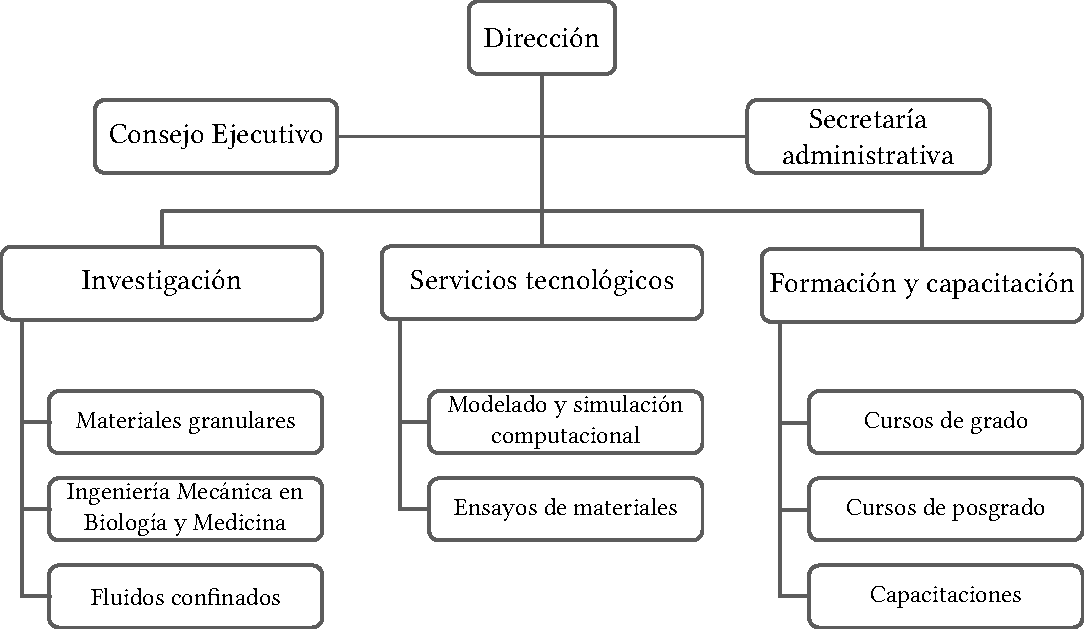
\includegraphics[width=0.7\textwidth]{estructura.pdf}
	      \end{center}
	      \begin{itemize}
		      \item \textbf{Responsable de área Investigación:} Marcos Madrid.
		      \item \textbf{Responsable de área Servicios Tecnológicos:} Martín Sánchez.
		      \item \textbf{Responsable de área formación y Capacitación:} Ariel Meyra.
	      \end{itemize}
\end{itemize}


\subsection{Objetivos y desarrollo}

Durante el año 2025, el Grupo de Materiales Granulares (GMG) tuvo como objetivo prioritario elaborar una propuesta de promoción a centro. Tal objetivo se cumplió exitosamente, culminando en el reconocimiento institucional del «Centro de Investigación en Mecánica Experimental y Computacional» (CIMEC) por medio de la Resolución N° 2461/2025 del Consejo Superior de la UTN.

Adicionalmente, los objetivos propuestos en el Plan de Trabajo 2025 fueron alcanzados en gran medida. La producción científica del grupo se sostuvo, alcanzando un número significativo de publicaciones en revistas con referato. La presentación de trabajos en reuniones científicas nacionales e internacionales fue similar a la correspondiente del año 2024, afectada principalmente debido a los altos costos y las severas restricciones presupuestarias. Todos los miembros del grupo han participado en la elaboración de trabajos que fueron publicados o comunicados a congresos y se mantuvieron los vínculos existentes con investigadores nacionales e internacionales a través de diversas colaboraciones.

El GMG organizó por cuarto año consecutivo el encuentro «PyDay La Plata» sobre el uso y aplicaciones del lenguaje de programación Python, y también el «III Workshop Granular» con la asistencia de colegas nacionales e internacionales.

Tres tesistas doctorales avanzaron en sus investigaciones sin mayores inconvenientes. Durante 2025 el grupo realizó tareas de formación en investigación por medio de becarios estudiantes financiados por la Universidad.

Finalmente, durante el año 2025 finalizaron exitosamente dos PID homologados por la Universidad, y se continuaron desarrollando las tareas PID vigentes.

En conclusión, durante el año 2025 el grupo mantuvo su funcionamiento y producción, cumpliendo con los objetivos planteados en el Plan de Trabajo.

\section{Personal}

\subsection{Nómina de investigadores}

{\small
	\begin{tabular}{l l l c c c}
		\toprule
		Apellido y nombre        & Cargos                     & Dedicación & Categ. UTN & Incentivos & Horas$^a$ \\
		\midrule
		Carlevaro, Carlos Manuel & Prof. Titular              & Simple     & B          & III        & 20        \\
		                         & Invest. Indep. CONICET     &            &            &            &           \\
		Fernández, Matías        & Prof. Adjunto              & Exclusiva  & D          &            & 30        \\
		                         & JTP                        & Simple     &            &            &           \\
		Irastorza, Ramiro Miguel & Prof. Titular              & Simple     & B          & III        & 15        \\
		                         & Invest. Indep. CONICET     &            &            &            &           \\
		Madrid, Marcos Andrés    & Prof. Adjunto              & Simple     & C          & III        & 15        \\
		                         & Invest. Asist. CONICET     &            &            &            &           \\
		Meyra, Ariel Germán      & Prof. Adjunto              & Simple     & C          & III        & 15        \\
		                         & Invest. Indep. CONICET     &            &            &            &           \\
		Sánchez, Martín          & Prof. Titular              & Simple     & B          &            & 15        \\
		Pilili, Esteban          & Jefe de Trabajos Prácticos & Simple     &            &            & 15        \\
		\bottomrule
	\end{tabular}
}

\normalsize
\vspace{0.5cm}
$^a$ Sólo se cuenta la dedicación a la investigación sin sumar aquí las horas dedicadas a la docencia o actividades de extensión.

\subsection{Personal profesional}
\begin{tabular}{l l l c c c}
	\toprule
	Apellido y nombre     & Cargos        & Dedicación & Categ. UTN   & Incentivos & Horas$^a$ \\
	\midrule
	García Ibarroule, Ruy & Ayud. Primera & Exclusiva  & (En trámite) &            & 15        \\
	\bottomrule
\end{tabular}

\normalsize
\vspace{0.5cm}
$^a$ Sólo se cuenta la dedicación a la investigación sin sumar aquí las horas dedicadas a la docencia o actividades de extensión.


\subsection{Personal técnico, administrativo y de apoyo}
No se cuenta con este tipo de personal.

% \begin{tabular}{l l r}
% \toprule
% Apellido y nombre & Horas \\
% \midrule
%  Villalba, Manuel &  40\\
%  \bottomrule
%  \end{tabular}

\subsection{Becarios y personal en formación}

\subsubsection{Tesistas de maestría y/o doctorado}
\begin{tabular}{l l l c l r}
	\toprule
	Apellido y nombre & Tipo de tesis        & Inicio  & Categ. UTN & Financ.            & Horas$^a$ \\
	\midrule
	Basiuk, Lucas     & Doc. Ing. Materiales & 10/2020 & F          & CONICET            & 40        \\
	Gracia, César     & Doc. Ing. Materiales & 4/2023  & G          & CONICET            & 40        \\
	Mosca, Santiago   & Doc. Ing. Materiales & 10/2020 & E          & Sin financiamiento & 5         \\
	\bottomrule
\end{tabular}

\normalsize
\vspace{0.5cm}
$^a$ Sólo se cuenta la dedicación a la investigación sin sumar aquí las horas dedicadas a la docencia o actividades de extensión.


\subsubsection{Becarios graduados}

El GMG no tuvo becarios graduados durante 2024.
%
%  \begin{tabular}{l l l l r}
%  \toprule
%  Apellido y nombre & Tipo de Beca & Financ. & Horas \\
%  \midrule
%  El Ahmar, Elías & Beca BINID & UTN & 20\\
%  \bottomrule 
%  \end{tabular}

\subsubsection{Becarios alumnos}

\begin{tabular}{l l l l r}
	\toprule
	Apellido y nombre   & Tipo de Beca & Financ. & Horas \\
	\midrule
	Curciarello, Thomas & Beca SCyT    & UTN     & 12    \\
	Köpke, Juan Ignacio & Beca SCyT    & UTN     & 12    \\
	Pellegrino, Eric    & Beca SAU     & UTN     & 12    \\
	Robert, Sara        & Beca SAU     & UTN     & 12    \\
	Zonco, Sofía        & Beca SCyT    & UTN     & 12    \\
	\bottomrule
\end{tabular}

\subsubsection{Pasantes}

Durante 2024 no hubo pasantes con tareas asignadas en el GMG.
% \begin{tabular}{l l r}
% \toprule
% Apellido y nombre & Financ. & Horas \\
% \midrule
% Vatalaro, Giancarlo & Sin financiamiento & 5\\
% \bottomrule
% \end{tabular}

\normalsize


\section{Equipamiento e infraestructura}

El CIMEC cuenta con dos oficinas, cinco laboratorios y un recinto climatizado para el cluster de cómputo. A continuación se enumeran los principales equipos y espacios disponibles.

\subsection{Equipamiento e infraestructura principal disponible}\label{sec:equipamiento}


\begin{itemize}
	\item Un clúster de cómputo dedicado con siete servidores Dell y seis servidores HP, ofreciendo un total de 156 unidades de procesamiento con 312 hilos administrados con SLURM, 336 GB de memoria RAM, 25 TB de almacenamiento y un nodo con GPU con 10.496 CUDA Cores, en una sala refrigerada de 4 m$^2$.
	\item Una celda de tipo Hele-Shaw con bomba peristáltica.
	\item Dos impresoras 3D.
	\item Un osciloscopio.
	\item Un analizador de redes vectorial.
	\item Dos placas adquisidoras.
	\item Dos balanzas electrónicas.
	\item Nueve computadoras de escritorio y para control de dispositivos de laboratorio.
	\item Una impresora láser B/N.
	\item Fuente regulada/regulable.
	\item Mobiliario básico de oficina y de laboratorio (escritorios, sillas, mesadas, mesas, armarios, etc.).
	\item Herramientas básicas (llaves, taladro, soldador, multímetro, etc.).
	\item Un banco de prueba para medición de tensiones en silos.
	\item Un agitador de varilla con conjunto soporte.
	\item Dos multímetros con termocupla tipo J.
	\item Dos cilindros de acrílico para estudio de silos.
	\item Dos notebooks ASUS con procesador Ryzen-7.
	\item Compresor de aire.
	\item Dos microscopios metalográficos de mesdada.
	\item Un microscopio metalográfico transportable.
	\item Un banco de desbaste.
	\item Una mufla para tratamientos térmicos hasta 950°C.
	\item Un durómetro Rocwell.
	\item Un durómetro Brinell.
	\item Dos durómetros de escalas combinadas Rocwell y Brinell.
	\item Un micro durómetro.
	\item Dos pulidoras metalográficas.
	\item Una cortadora metalográfica refrigerada.
	\item Dos lijadoras de banda refrigeradas.
	\item Material de vidrio de laboratorio.
	\item Un yugo magnético con insumos.
	\item Una lámpara de luz ultravioleta con insumos.
	\item Una máquina de ensayos Charpy e Izod.
	\item Una fuente de corriente continua regulable.
	\item Generador de funciones digital.
	\item Fuente de corriente continua regulable digital.
\end{itemize}

\subsection{Oficinas y sala}

\begin{itemize}
	\item {\bf Oficina:} Dos oficinas de 22 m$^2$ cada una.
	\item {\bf Cluster:} Sala de 4 m$^2$.
\end{itemize}

\subsection{Laboratorios y talleres}

\begin{itemize}
	\item {\bf Laboratorio A:} Laboratorio de 20 m$^2$.
	\item {\bf Laboratorio B:} Laboratorio de 6 m$^2$.
	\item {\bf Laboratorio C:} Laboratorio de 22 m$^2$.
	\item \textbf{Laboratorio de Automatización Industrial:} de 35 m$2$.
	\item \textbf{Laboratorio de Materiales Metálicos y Tratamientos Térmicos} de 50 m$2$.
\end{itemize}

\subsection{Servicios generales}

\begin{itemize}
	\item {\bf Centro de mecanizado:} Servicio prestado por el Departamento de Ing. Mecánica.
	\item {\bf Talleres:} Servicio prestado por el Departamento de Ing. Mecánica.
	\item {\bf Biblioteca:} Servicio prestado por la Facultad Regional La Plata, y por la biblioteca propia del Departamento de Ingeniería Mecánica. Adicionalmente se cuenta con el servicio de biblioteca electrónica del Min. de Ciencia, Tecnología e Innovación Productiva.
\end{itemize}

\subsection{Cambios significativos en el período}

Como consecuencia de la formalización del centro, el mismo se constituyó sumando a las instalaciones y equipamiento del GMG los laboratorios de Automatización Industrial, de Materiales Metálicos y Tratamientos Térmicos y el que fue utilizado en estudios de calidad de aire.

Estas incorporaciones sumaron, además de los espacios respectivos, nuevos equipamientos que aparecen listados en la sección \ref{sec:equipamiento}.

\section{Documentación y biblioteca}

El CIMEC cuenta con una reducida biblioteca que incluye principalmente actas de congresos y libros de resúmenes de eventos científicos en los que han participado sus investigadores, como así también manuales de los instrumentos adquiridos. El material de consulta bibliográfico es mantenido por la biblioteca de la Facultad Regional La Plata, el Departamento de Ingeniería Mecánica y la biblioteca electrónica del Ministerio de Ciencia Tecnología e Innovación Productiva.

\chapter{Actividades I+D+i}

\section{Investigaciones}

\subsection{Proyectos en curso}

\begin{itemize}

	\item {\bf PID UTN:} MAUTNLP0009875, 2023-2025, {\bf Propiedades estructurales en carga y descarga de silos}. Director: Marcos Madrid, codirector: Manuel Carlevaro. {\color{red} Actualizar 2025}

		      {\bf Objetivos:} el objetivo general consiste en avanzar sobre la comprensión de los fenómenos que ocurren durante la manipulación de materiales granulares y su aplicación para mejorar tanto los procesos como los diseños y construcción. Como objetivos particulares proponemos: a) predecir la presión en el interior de un silo durante la carga y descarga para diferentes protocolos de llenado; b) predecir las presiones en el interior de un silo reforzado con tensores en diferentes configuraciones durante la carga y descarga del mismo.

		      {\bf Logros:} En el año 2024, se avanzó en la construcción, puesta a punto y una primera etapa de mediciones de un silo a escala tanto con como sin obstáculos y se contrastaron resultados con simulaciones

		      {\bf Dificultades:} no se produjeron dificultades en el desarrollo del proyecto.

	\item {\bf PID UTN:} MAECLP0009851TC, 2023-2026, {\bf Resolución de problemas Biomédicos y Biomiméticos por Elementos Finitos}. Director: Ramiro M. Irastorza.

		      {\bf Objetivos:} El objetivo general de la investigación es desarrollar y poner a punto la metodología para la resolución de problemas mediante el Método de Elementos Finitos, principalmente relacionados con la Ingeniería Mecánica y con geometrías complejas y de gran cantidad de elementos. Se trabajará construyendo geometrías a partir de reconstrucciones tomográficas, lo cual constituye un importante desafío dado que generalmente los archivos STL provenientes de los programas de recontrucción no son los adecuados para la simulación por elementos finitos. Se atacarán problemas con el Método de Elementos Finitos en dos aplicaciones: (i) ablación por medio de energía electromagnética y (ii) biomecánica. Respecto del tema (i): 1. Desarrollar modelos de torso completo para la simulación de ablación por radiofrecuencia aplicado a arritmias cardíacas. 2. Se propone estudiar por simulación la técnica de campo eléctrico pulsado (PEF). En esta técnica se busca el efecto de electroporación, y el daño provocado no es térmico, si no eléctrico. Objetivos particulares del tema (ii): 3. Relacionados con el procedimiento de discoplastía, el objetivo es construir geometrías de pacientes “tipo” a partir de tomografías o resonancias magnéticas y evaluar de manera cuantitativa distancias, superficies, volúmenes, y ángulos de los dominios a simular. Se espera concluir y obtener mediciones más controladas que las tomadas en dos dimensiones por los médicos. 4. Continuando con el objetivo anterior, se propone simular el par de vértebras lumbares L4 y L5 (las más afectadas en estos casos) y estudiar los modelos mecánicos que se aplican a estos tejidos. Al poseer imágenes pre y pos operación (con implante de PMMA), es posible realizar simulaciones en las dos condiciones y evaluar las diferencias en tensiones, deformaciones y desplazamientos. Finalmente, un objetivo importante en este proyecto es consolidar un grupo multidisciplinario de investigación dedicado a la simulación utilizando Métodos de Elementos Finitos en general, y en particular en aplicaciones biomédicas, biológicas y biomiméticas.

	      {\bf Logros:} se desarrolló un modelo simplificado de torso, basado en geometrías porcinas, que mostró una influencia moderada del tamaño corporal en el efecto del parche dispersivo, siendo más relevante en individuos pequeños. Por otro lado, experimentalmente, se observó que la radiofrecuencia en tejido desecado genera coagulación hasta 3 mm, y que potencias medias son más eficaces que altas. El monitoreo de la corriente de RF permite optimizar la potencia aplicada. Finalmente, se continuó trabajando en termocoagulación de zonas epileptógenas (con modelos realistas construidos a partir de imágenes de cerebro), en particular, en heterotopía periventricular. Se concluyó que no se muestra una alteración de la zona de coagulación debido a la proximidad del ventrículo. Se publicaron dos trabajos en revistas internacionales en esta temática y dos trabajos completos en el congreso de la Sociedad Argentina de Bioingeniería (SABI 2025). En la temática de biomecánica, se desarrolló un modelo simplificado por elementos finitos que permite simular condiciones fisiológicas y patológicas del disco intervertebral (cambios en la altura del disco, el volumen del núcleo pulposo y la cantidad de cemento óseo inyectado). El resultado se publicó como trabajo completo en las actas de la Asociación Argentina de Mecánica Computacional. Finalmente, se trabajó en el modelado de la conductividad eléctrica en hueso cortical en función de su microestructura y anisotropía. Este modelo también fue presentado en SABI 2025.

		      {\bf Dificultades:} no se produjeron dificultades en el desarrollo del proyecto.


	\item \textbf{PID UTN:} MATCLP10087C, 2024--2027, \textbf{Estudio de propiedades dinámicas y estructurales de materiales granulares}. Director: Manuel Carlevaro.

	      \textbf{Objetivos:} El objetivo general del presente proyecto consiste en contribuir al conocimiento, tanto básico como aplicado, relativo a las características y comportamiento de la materia granular en procesos dinámicos de flujo y transporte, en sistemas de interés en procesos industriales y tecnológicos. Si bien el comportamiento de la materia granular en procesos y dispositivos tecnológicos es muy diverso y complejo, se abordará la descarga de silos en dos y tres dimensiones, el transporte de material granular en fracturas angostas y el fenómeno de amortiguamiento mediante materiales granulares.

	      \textbf{Logros:} Analizando el transporte de material granular en fractuas planas, se compararon mezclas binarias con sistemas monodispersos, manteniendo siempre el mismo diámetro promedio para aislar el efecto de la variedad dimensional. Los resultados revelan que la permeabilidad y la conductividad permanecen prácticamente inalteradas, incluso cuando existe una mezcla de diferentes medidas. Sin embargo, el análisis destaca que las partículas de mayor tamaño soportan tensiones mecánicas superiores, lo que las vuelve más vulnerables al aplastamiento. Como conclusión, el estudio sugiere que aumentar el tamaño medio de los granos es más efectivo para mejorar el flujo que intentar reducir la dispersión de sus dimensiones. Respecto del análisis de amortiguadores granulares, se completó la fase de desarrollo de un prototipo experimental para el estudio del efecto de la forma del contenedor en la respuesta mecánica del sistema vibrante.

	      \textbf{Dificultades:} No se presentaron dificultades durante el año 2025.

	\item \textbf{PID UTN:} ENECLP0010122, 2024--2027, \textbf{Incidencia de la viscosidad del fluido en el transporte del agente de sostén dentro de una fractura de yacimiento no convencional}. Director: Matías Fernández. {\color{red} Actualizar 2025}

	      \textbf{Objetivos:} El objetivo general de este proyecto es mejorar los procesos de estimulación por fractura hidráulica estudiando la forma en que penetra y se deposita el agente de sostén durante la fractura. Se espera que este conocimiento ayude a diseñar protocolos de fracturación que consigan una disposición de los agentes de sostén dentro de las fracturas que den mayor estabilidad (vida útil) y mayor conductividad (producción).

	      \textbf{Logros:} Se realizó el mantenimiento general al equipo de fractura del laboratorio: Cambios de válvulas y tanque de desagüe; sellado de las paredes del equipo y cambio de junta elastómera; cambio de fluido de bomba peristáltica. Se logró realizar la ingeniería de detalle de un viscosímetro automatizado para la caracterización de fluidos.

	      \textbf{Dificultades:} Los costos han aumentado de manera significativa, por lo que impactó en el plan de trabajo propuesto y demoras en las compras realizadas.

\end{itemize}

\subsection{Tesis}

Se encuentran en desarrollo tres trabajos de tesis doctoral:
\begin{itemize}
	\item Santiago Mosca: ``Modelización de flujo y transporte en medios porosos''. Director: Manuel Carlevaro. Codirector: Federico Castez (Y-TEC, UNLP).
	\item Lucas Osvaldo Basiuk: ``Diseño computacional de matrices para ingeniería de tejidos optimizadas de manera estocástica''. Director: Manuel Carlevaro. Codirector: Ramiro Irastorza.
	\item César Gracia: ``Incidencia de las características reológicas de un fluido de fractura en el transporte y sedimentación del agente de sostén en estimulación hidráulica de yacimientos''. Director: Manuel Carlevaro. Codirector: Matías Fernández.
\end{itemize}

\subsection{Trabajos publicados}

\subsubsection{Con referato}

\begin{enumerate}
	\item \fullcite{GMG-081}.
	\item \fullcite{GMG-082}.
	\item \fullcite{GMG-083}.
	\item \fullcite{GMG-084}.
	\item \fullcite{GMG-085}.
	\item \fullcite{GMG-086}.
	\item \fullcite{GMG-089}.
\end{enumerate}

\subsubsection{Sin referato}
No se publicaron trabajos sin referato.

\subsection{Congresos y reuniones científicas}

\subsubsection{Trabajos completos con referato}
\begin{enumerate}
	\item \fullcite{GMG-090}.
	\item \fullcite{GMG-091}.
	\item \fullcite{GMG-092}.
	\item \fullcite{GMG-093}.
\end{enumerate}

\subsubsection{Presentaciones sin referato}

\begin{enumerate}
	\item \fullcite{2025-01}.
	\item \fullcite{2025-02}.
	\item \fullcite{2025-03}.
	\item \fullcite{2025-04}.
	\item \fullcite{2025-05}.
\end{enumerate}

\subsubsection{En libros y capítulos de libros}

\begin{enumerate}
	\item F. Batista y Manuel Carlevaro. \textbf{Python para Ciencia y Tecnolgía}, 2025. Autoeditado, ISBN:  978-631-00-9794-7. \url{https://libropython.science/}.
\end{enumerate}

\subsubsection{Informes y memorias técnicas}
\begin{enumerate}
	\item Memoria anual del GMG para el período 2024 (ISSN: 2618-1738).
\end{enumerate}
\vspace{0.25cm}

\section{Organización}
\subsection{PyDay La Plata 2025}

El grupo organizó el «PyDay La Plata 2025», con el apoyo de la Asociación Civil Python Argentina\footnote{\url{https://ac.python.org.ar/}}. Este evento se realizó el día 8 de noviembre en el Salón de Actos ``Presidente Juan Domingo Perón'' de la Facultad Regional La Plata, y contó con la presencia de aproximadamente un centenar de asistentes que participaron en las ocho charlas programadas. Los títulos de Las charlas y sus correspondientes expositores, fueron las siguientes:
\begin{itemize}
	\item \textit{Python como herramienta de exploración, automatización y aprendizaje}, Lautaro.
	\item \textit{DevSecOps automatizados aplicado a proyectos reales}, Jonathan Santurio e Iñaki Sarobe.
	\item \textit{¡En mi máquina funcionaba! Las trampas de Python al pasar de Windows a Linux}, Jorge Ronconi.
	\item \textit{El origen de la programación}, Fabian Martinez Rincon.
	\item \textit{Del Cálculo Numérico a la automatización de gráficas de fasores con Python}, Diego Amiconi y Santiago Hernández.
	\item \textit{Del laboratorio al código: análisis del envejecimiento a corto plazo de asfaltos mediante python}, Johanna Peters y Benjamin Esteban Sioma.
	\item \textit{Microscopía cuantitativa con Python: la importancia de la automatización y el código abierto}, Carla Soprano.
	\item \textit{Procesamiento Paralelo de Vectores}, Facundo Batista.
\end{itemize}

Adicionalmente se brindaron charlas relámpago de 5 minutos, abiertas al público. Además del apoyo institucional de la FRLP, el evento contó con el patrocinio de las empresas: SysArmy, Lovelytics, Tecsolve S.R.L. y Gcoop.

\subsection{III Workshop Granular}
El GMG organizó por tercera vez el «III Workshop Granular» que se llevó a cabo el 18 de septiembre, en la Biblioteca de la Facultad Regional La Plata de la UTN.

El encuentro contó con la participación de investigadores y estudiantes de la Facultad de Ciencias Exactas y Naturales de la Universidad Nacional de La Pampa, de la Facultad de Ingeniería de la Universidad de Buenos Aires, del Instituto Tecnológico de Buenos Aires, de la Universidad de La República de Uruguay y del GMG, sumando un total de 24 asistentes y expositores. El evento consistió en las siguientes charlas:
\begin{itemize}
	\item Thomas Gallot (Universidad de la República, charla invitada): \textit{Soft Granular Media for Laboratory Scale Experiments}.
	\item Camila Sedofeito (Universidad de la República): \textit{Memory in Granular Media Under Loading Cycles}.
	\item Juan Köpke (GMG – FRLP): \textit{Eficiencia de elevadores sinfín en función del ángulo}.
	\item Thomas Curciarello (GMG – FRLP): \textit{Amortiguador granular GMG}.
	\item Daniel Parisi (Instituto Tecnológico de Buenos Aires, charla invitada): \textit{Modelos de Partículas Autopropulsadas con Deformación Activa inspirados en Linfocitos T}.
	\item Fabricio Fernández (Facultad de Ingeniería – UBA): \textit{Fenómenos críticos en la dinámica de flujos cargados de partículas}.
	\item Sofía Zonco (GMG – FRLP): \textit{Influencia de la rugosidad de paredes en el flujo de particulas en silos 2D}.
	\item Luis Pugnaloni (Facultad de Ciencias Exactas y Naturales – UNLPam, charla invitada): \textit{Flujo de granulares por orificios inclinados}.
\end{itemize}



\section{Actividades de gestión y evaluación}

Los miembros del CIMEC participan además en las siguientes actividades académicas y de gestión:

\begin{itemize}
	\item \textbf{Director del Departamento de Ingeniería Mecánica:} Matías Fernández se desempeñó como Director de Departamento durante el año 2025.

	\item \textbf{Consejo Asesor de Ciencia Tecnología y Postgrado UTN-FRLP:} Ramiro Irastorza fue miembro de la comisión durante 2025.

	\item \textbf{Comisión de Posgrado:} Ariel Meyra fue miembro de esta Comisión en 2025.

	\item \textbf{Referato de artículos para revistas internacionales}: durante 2025, C. Manuel Carlevaro fue revisor de artículos para la revista \textit{Journal of Statistical Mechanics - Theory and Experiment} (IOP) y \textit{Scientific Reports} (Nature Research).

	\item \textbf{Actividades de gestión editorial:} C. Manuel Carlevaro fue Editor Asociado de \textit{Frontiers in Soft Matter}.

	\item \textbf{Evaluación de personal de CyT}: C. Manuel Carlevaro fue Especialista Externo en la evaluación de la Convocatoria Promoción CIC 2024 de CONICET. Marcos Madrid fue miembro evaluador de la Carrera del Personal de Apoyo de CONICET.

	\item \textbf{Jurados de tesis}: Ramiro M. Irastorza fue miembro del jurado evaluador de la tesis doctoral de Matías Oliva (Facultad de Ingeniería Universidad Nacional de La Plata). También fue jurado del proyecto final de carrera de Sofía Díaz (Instituto de Medicina Traslacional e Ingeniería Biomédica de la Universidad Hospital Italiano de Buenos Aires).


	      % \item \textbf{Jurados de concursos docentes}: C. Manuel Carlevaro fue miembro titular del jurado del concurso para cargos de Profesor de la asignatura «Procesos Industriales» realizado en el Departamento de Ingeniería Mecánica, de la Facultad Regional La Plata de la Universidad Tecnológica Nacional.

	      % \item \textbf{Evaluación de proyectos de CyT}: C. Manuel Carlevaro fue evaluador de PICT de la Agencia Nacional de Promoción Científica y Tecnológica, en el área temática ``Tecnología Informática de las Comunicaciones y Electrónica''. R. Irastorza se desempeñó como Co-Coordinador de la comisión de Tecnología Informática, de las Comunicaciones y Electrónica en la evaluación de Proyectos PICT de la Agencia Nacional de Promoción Científica y Tecnológica (ANPCYT); Ministerio de Ciencia, Tecnología e Innovación Productiva. 

	\item \textbf{Asociación Física Argentina:} C. Manuel Carlevaro se desempeñó como Revisor de Cuentas Suplente. Marcos Madrid fue parte del comité ejecutivo de la división Materia Blanda.

\end{itemize}


\section{Otras actividades}

\subsection{Visitas recibidas y realizadas}

\subsubsection{Visitantes recibidos}

\begin{itemize}
	\item \textbf{Lou Kondic:} julio. Investigador del \textit{New Jersey Institute of Technology}, Estados Unidos.
	\item {\bf Luis Pugnaloni:} septiembre. Investigador de la Universidad Nacional de La Pampa.
	\item \textbf{Enrique Berjano:} octubre. Investigador de la Universidad Politécnica de Valencia, España.
\end{itemize}

\subsubsection{Visitas realizadas}

\begin{itemize}
	\item \textbf{Lucas Basiuk:} diciembre -- marzo (2026) Investigador visitante en la Universidad de Salerno, Italia.
	      % \item {\bf Manuel Carlevaro:} enero--abril. Investigador visitante en la Universidad de Navarra, Pamplona, España.
\end{itemize}


\subsection{Tareas de divulgación}
Los integrantes del GMG participamos de las siguientes actividades de divulgación:

\begin{itemize}
	\item Ramiro Irastorza participó como expositor en las Jornadas de Formación Profesional de la UTN, el 15 de mayo de 2025. Título de charla: "Elementos Finitos e Inteligencia Artificial: ¿La Nueva Era de la Ingenierı́a?".
\end{itemize}

\section{Registros y patentes}

No se realizaron registros ni patentes.


\chapter{Actividades en docencia}

\section{Docencia de grado}

Los integrantes del CIMEC se desempeñaron como docentes de las siguientes cátedras de la UTN-FRLP.

\begin{itemize}
	\item {\bf Estimulación hidráulica de yacimientos no convencionales:} M. E. Fernández.
	\item {\bf Introducción a los elementos finitos:} R. Irastorza.
	\item {\bf Fundamentos de Informática:} M. Madrid.
	\item {\bf Cálculo Avanzado:} Manuel Carlevaro.
	\item \textbf{Estabilidad II:} L. Basiuk.
	\item \textbf{Materiales no metálicos:} A. Meyra.
\end{itemize}


\section{Posgrado}

Los docentes del GMG son docentes en los siguientes cursos de postgrado.

\begin{itemize}
	\item {\bf Herramientas computacionales para científicos:} R. Irastorza. A. Meyra y C. M. Carlevaro.
	\item \textbf{Método de elementos finitos con software libre:} R. Irastorza y A. Meyra.
	\item \textbf{Estimulación hidráulica de yacimientos no convencionales:} M. Fernández.
	\item {\bf Análisis Estadístico utilizando R (Universidad Nacional Arturo Jauretche):} R. Irastorza.
\end{itemize}

\section{Otras actividades}

El banco de pruebas de descarga de silos montado en los laboratorios del GMG se utiliza para que estudiantes de las cátedras de grado realicen trabajos prácticos experimentales sobre flujo de materiales granulares y distribución de tensiones en un silo.


% M. Fernández fue integrante del Tribunal Evaluador de Proyecto Final de carrera de:
% \begin{itemize}
% 	\item Juan Pablo Bustos: «Toma de fuerza y actuación hidráulica autónoma en tolva autodescargable».
% 	\item Matías Nicolás Gómez: «Carro manual de carga de dos ruedas».
% \end{itemize}

\chapter{Vinculación con el medio socioproductivo}

\section{Transferencia al medio socioproductivo}

Integrantes del GMG participan del consorcio de Corrosión Microbiológica (MIC II) llevado adelante por Y-TEC desarrollando un modelo de simulación computacional que implementa la interacción de poblaciones de bacterias en aplicaciones de gas \& oil.

L. Basiuk, M. Carlevaro, R. Irastorza, M. Madrid y A. Meyra participaron de la prueba piloto de la iniciativa Consorcio Agro.ar titulada \textit{Ensayos computacionales de transporte granular en sinfín} (ver en [1] un resumen técnico de lo desarrollado). En esta prueba se trabajó en conjunto con el Centro Tecnológico CIDETER y las empresas del sector: Mainero y CIA SAICFI y silos D’ascanio SRL. El trabajo realizado permitió caracterizar sistemáticamente el comportamiento del transporte por sinfín, identificando parámetros clave para su optimización y proponiendo mejoras concretas en el diseño y la operación. Los modelos desarrollados y los resultados obtenidos sientan las bases para futuras colaboraciones tendientes a maximizar la eficiencia y minimizar el daño granular en equipos de transporte agroindustrial.

	[1] Basiuk L. O., Carlevaro C. M., Irastorza R. M., Madrid M. A., Meyra A.G. \textbf{Agro.AR Ciencia Aplicada: por qué y cómo innovar en la agroindustria}, ISSN en línea 2718-6660, Vol. 6, N.° 3, noviembre 2025, Revista MDA, Publicación del Ministerio de Desarrollo Agrario de la Provincia de Buenos Aires.


\chapter{Informe sobre rendición general de cuentas}

Los valores presentados en la siguiente tabla son estimativos debido a que existen ingresos y erogaciones correspondientes a períodos diferentes del año 2024 dependiendo del inicio y cierre de los subsidios recibidos.

\vspace{1cm}
% Gastos capital: Inciso 4.3
% Gastos corrientes: Incisos 2 + 3
\begin{center}
	\begin{tabular}{ l c c c }
		\toprule
		\textbf{Proyecto} & \textbf{Ingresos (\$)} & \multicolumn{2}{c} {\textbf{Egresos (\$)}}                       \\
		                  &                        & \textbf{Capital}                           & \textbf{Corrientes} \\
		\midrule
		UTN$^a$           & 1.800.000,00           & 1.000.000,00                               & 337.733,95          \\
		MAUTNLP0009875    & 1.080.000,00           & 518.000,00                                 & 240.000,00          \\
		MAUTCLP10087C     & 1.260.000,00           & 600.000,00                                 & 268.924,76          \\
		MAECLP0009851TC   & 1.080.000,00           & 759.085,00                                 & 123129.95           \\
		ENECLP0010122     & 1.080.000,00           & 306.606,14                                 & 0,00                \\
		\midrule
		\textbf{Total:}   & 6.300.000,00           & 3.183.691,14                               & 969.788,66          \\
		\bottomrule
	\end{tabular}
\end{center}

\vspace{0.5cm}
$^a$ Financiamiento de la SCTyP de la UTN para grupos homologados.


\chapter{Programa de actividades 2026}

El año 2026 será el primer año de funcionamiento del CIMEC, por lo que la planificación de actividades se agruparán en forma lógica por cada área.

\section{Área de Investigación}

Se continuará con el normal desarrollo de los proyectos financiados en ejecución:

\begin{itemize}
	\item PID: MAUTNLP0009875. Se continuará con las mediciones experimentales de presión en la base de los silos prototipo, y se construirán dos nuevos modelos complementarios para realizar experimentos con paredes de diferentes rugosidades. {\color{red} Actualizar a 2026}
	\item PID: MAECLP0009851TC. Dado que el proyecto está finalizando se continuarán los trabajos asociados a la termocoagulación de zonas epileptógenas y se explorarán métodos de electroporación en diferentes tipos de cancer. Adicionalmente, continuaremos con la simulación de la biomecánica de columna con discoplastía y otras técnicas asociadas a la estabilidad de la misma.
	\item PID UTN MATCLP10087C: Se avanzará en el análisis de la descarga de un silo en dos dimensiones sometido a vibraciones bi-armónicas por medio de simulaciones computacionales. Se finalizará el desarrollo del dispositivo experimental para el estudio de vibraciones granulares.
	\item PID ENECLP0010122: Se caracterizarán diferentes propiedades reológicas de fluidos y sus efectos en el transporte de material granular dentro de una celda de ensayo de fracturas. {\color{red} Actualizar a 2026}
\end{itemize}

En términos generales, son objetivos para el 2026:
\begin{itemize}
	\item  Redactar y publicar al menos siete trabajos en revistas internacionales con referato, producto de las investigaciones en las líneas de trabajo actualmente en desarrollo en el GMG.
	\item  Participar en al menos tres congresos nacionales y uno internacional.
	\item  Progresar en el desarrollo de los planes de tesis doctorales en curso.
	\item  Avanzar en la consolidación de las líneas de trabajo de los investigadores jóvenes.
	\item  Incorporar becarios estudiantes y graduados.
	\item  Continuar y consolidar las colaboraciones existentes con organismos nacionales e internacionales.
	\item  Participar en las actividades que proponga la Secretaría de Ciencia y Tecnología de la Facultad Regional La Plata.
\end{itemize}

\section{Área de Servicios Tecnológicos}
Se continuará la participación en el consorcio de Corrosión Microbiológica (MIC II) de la empresa Y-TEC desarrollando modelos computacionales de poblaciones bacteriales para aplicaciones de Gas \& Oil.

Por otra parte, se seguirán las gestiones para proveer servicios a empresas del sector agroindustrial relacionados con el estudio de procesos que involucren el almacenamiento y transporte de material granular.

\section{Área de Formación y Capacitación}

Se mantendrá la oferta de cursos de posgrado homologados para el doctorado, y se evaluará la posibilidad de ofrecer cursos de diplomatura.

\end{document}

